\documentclass[12pt,a4paper]{article}
\usepackage{fancyhdr} % Required to customize headers
\pagestyle{fancy}
\usepackage[portuguese]{babel}
\usepackage[utf8]{inputenc}
\usepackage[T1]{fontenc}
\usepackage{textcomp}
\usepackage{xcolor} % Pacote para cores
\usepackage{xspace} % Adiciona suporte para espaçamento inteligente
\usepackage{graphicx} % Para incluir imagens
\usepackage{pdfpages} % Para incluir arquivos PDF
\usepackage[left=2.48cm,right=1.7cm,top=2.35cm,marginparwidth=3.4cm]{geometry}
%\usepackage{lipsum} % Para gerar texto de exemplo
%\renewcommand{\headrulewidth}{0pt}
% Defina o caminho para o logotipo da universidade
\newcommand{\universitylogo}{imagens/logo_uerj_cor.jpg}
\fancyheadoffset[L]{2mm}
\renewcommand{\headrulewidth}{0pt} % Remove a linha horizontal no cabeçalho
% Pacotes de hiperlinks
\usepackage{hyperref}
\hypersetup{
	colorlinks,
	citecolor=blue,
	filecolor=magenta,
	linkcolor=blue,
	urlcolor=cyan
}

% Configurar o cabeçalho apenas para a primeira página
\fancypagestyle{firstpage}{
  \fancyhf{} % Limpar os estilos padrão

  % logo e Nome da universidade
  \lhead{
    \begin{minipage}{0.15\textwidth}
      \includegraphics[width=2.5cm]{\universitylogo}
    \end{minipage}
    \hfill
    \begin{minipage}{0.85\textwidth} % Ajuste o tamanho conforme necessário
      \raggedright % Alinha o texto à esquerda
      UNIVERSIDADE DO ESTADO DO RIO DE JANEIRO \\
      CENTRO DE TECNOLOGIA E CIÊNCIAS \\
      FACULDADE DE ENGENHARIA \\
      DEPARTAMENTO DE ENGENHARIA DE SISTEMAS E COMPUTAÇÃO \\
    \end{minipage}
  }
}
% Remover cabeçalho das outras páginas
%\pagestyle{plain} % Define o estilo das páginas subsequentes como básico (sem cabeçalho)

% Pacotes de formatação e layout


\title{Documentos Oficiais}

\begin{document}
\thispagestyle{firstpage} % Aplica o cabeçalho na primeira página
\headsep = 20pt
\setlength{\parindent}{0cm} % Remove paragraph indentation
\setlength{\tabcolsep}{5pt} % Espaço horizontal
\vspace*{2.0cm}

A seguinte documentação oficial relativa ao processo de reforma curricular encontra-se apensada nas
páginas a seguir:

\begin{enumerate}
      \item \textbf{Câmara de Educação Superior do Conselho Nacional de Educação}  \\
            \textbf{RESOLUÇÃO CNE/CES n\textordmasculine{}~5, DE 16 DE NOVEMBRO DE 2016} \\
            Institui as Diretrizes Curriculares Nacionais para os cursos de graduação na área da Computação, abrangendo os cursos de bacharelado em Ciência da Computação, em Sistemas de Informação, em \textbf{Engenharia de Computação}, em Engenharia de Software e de licenciatura em Computação, e dá outras providências (pág.~\pageref{cne2016}).

      \item \textbf{Sociedade Brasileira de Computação (SBC)}  \\
            \textbf{Referenciais de Formação para os Cursos de Graduação em Computação –-- 2017} \\
            Documento elaborado com base na Resolução CNE/CES n\textordmasculine{}~5/2016, com o objetivo de orientar a estrutura curricular dos cursos da área de Computação, considerando competências, conteúdos e práticas pedagógicas atualizadas (pág. \pageref{sbc2017}).

      \item \textbf{Câmara de Educação Superior do Conselho Nacional de Educação} \\
            \textbf{RESOLUÇÃO n\textordmasculine{}~7, DE 18 DE DEZEMBRO DE 2018} \\
            Estabelece as Diretrizes para a Extensão na Educação Superior Brasileira e regimenta o disposto na Meta 12.7 da Lei n\textordmasculine{}~13.005/2014, que aprova o Plano Nacional de Educação –-- PNE –-- 2014-2024 e dá outras providências (pág. \pageref{rcne2018}).

      \item \textbf{Universidade do Estado do Rio de Janeiro}  \\
            \textbf{Deliberação n\textordmasculine{}~33, DE 28 DE DEZEMBRO DE 1995} \\
            Dispõe sobre as Normas Gerais de Ensino de Graduação da UERJ (pág. \pageref{delib3395}).

      \item \textbf{Universidade do Estado do Rio de Janeiro}  \\
            \textbf{Deliberação n\textordmasculine{}~59, DE 12 DE DEZEMBRO DE 2019} \\
            Altera o Capítulo II, artigos 56, 57 e seu parágrafo único, da Deliberação n\textordmasculine{}~33/1995, que trata das normas gerais de Ensino de Graduação da UERJ (pág. \pageref{delib592019}).
      \item \textbf{Universidade do Estado do Rio de Janeiro}  \\
            \textbf{Deliberação n\textordmasculine{}~04, DE 13 DE ABRIL DE 2023}  \\
            Dispõe sobre a inserção curricular da extensão nos cursos da UERJ e dá outras providências (pág. \pageref{del4}).
      \item \textbf{CONFEA – Conselho Federal de Engenharia e Agronomia} \\
            \textbf{RESOLUÇÃO n\textordmasculine{}~380, DE 17 DE DEZEMBRO DE 1993}  \\
            Discrimina as atribuições provisórias dos Engenheiros de Computação ou Engenheiros Eletricistas com ênfase em Computação e dá outras providências. Brasília: Diário Oficial da União, Seção I, página 193, 06 de janeiro de 1994 (pág. \pageref{confea1993}).
\end{enumerate}
% Insere quebra de página
\newpage
\pagestyle{empty}
\thispagestyle{empty}
% Legislação
% Institui as Diretrizes Curriculares Nacionais para os cursos de graduação na área da Computação
\section{Resolução CNE/CES n\textordmasculine{} 5, de 16 de novembro de 2016}
\label{cne2016}
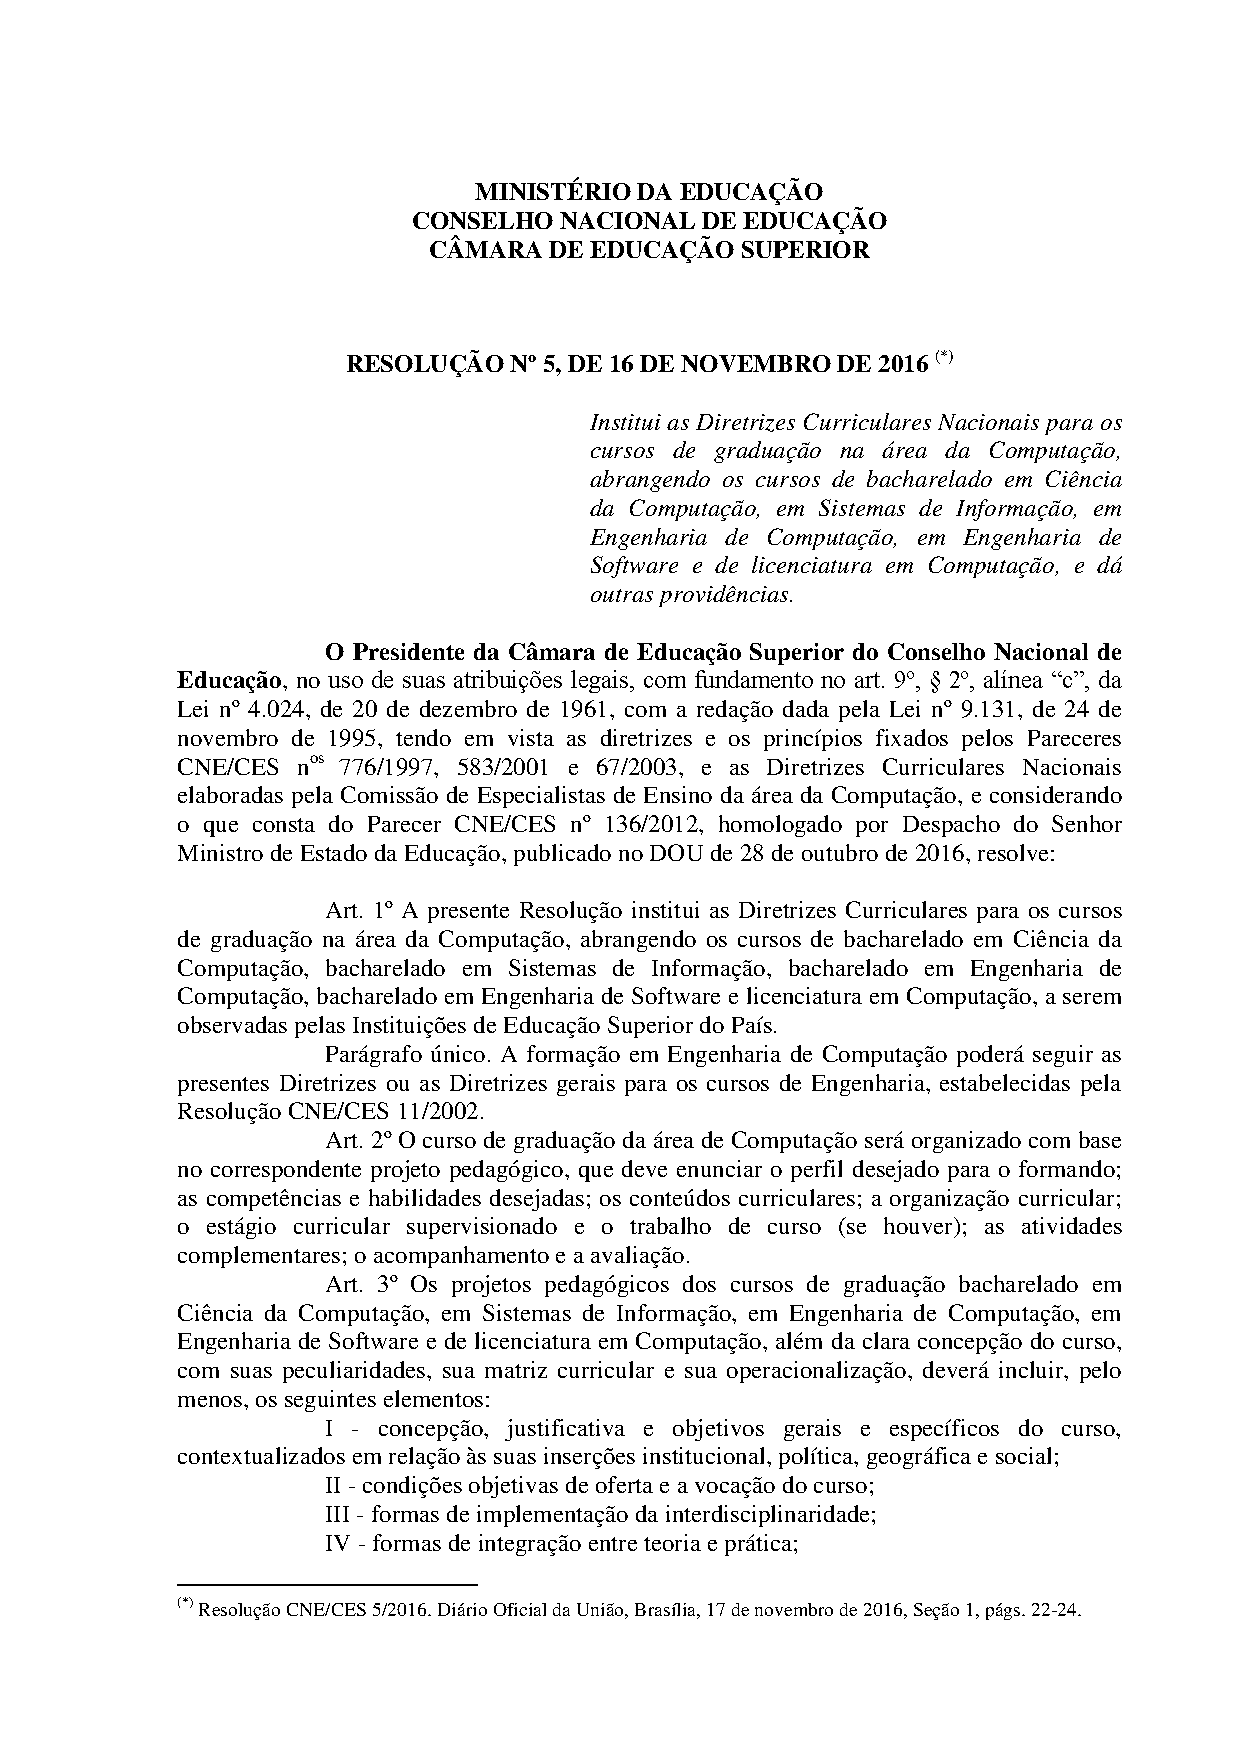
\includepdf[pages=-,pagecommand={\thispagestyle{empty}}]{leis/rces005_16.pdf}
% Referenciais SBC para cursos de Computação
\section{SBC: Referenciais para Graduação em Computação}
\label{sbc2017}
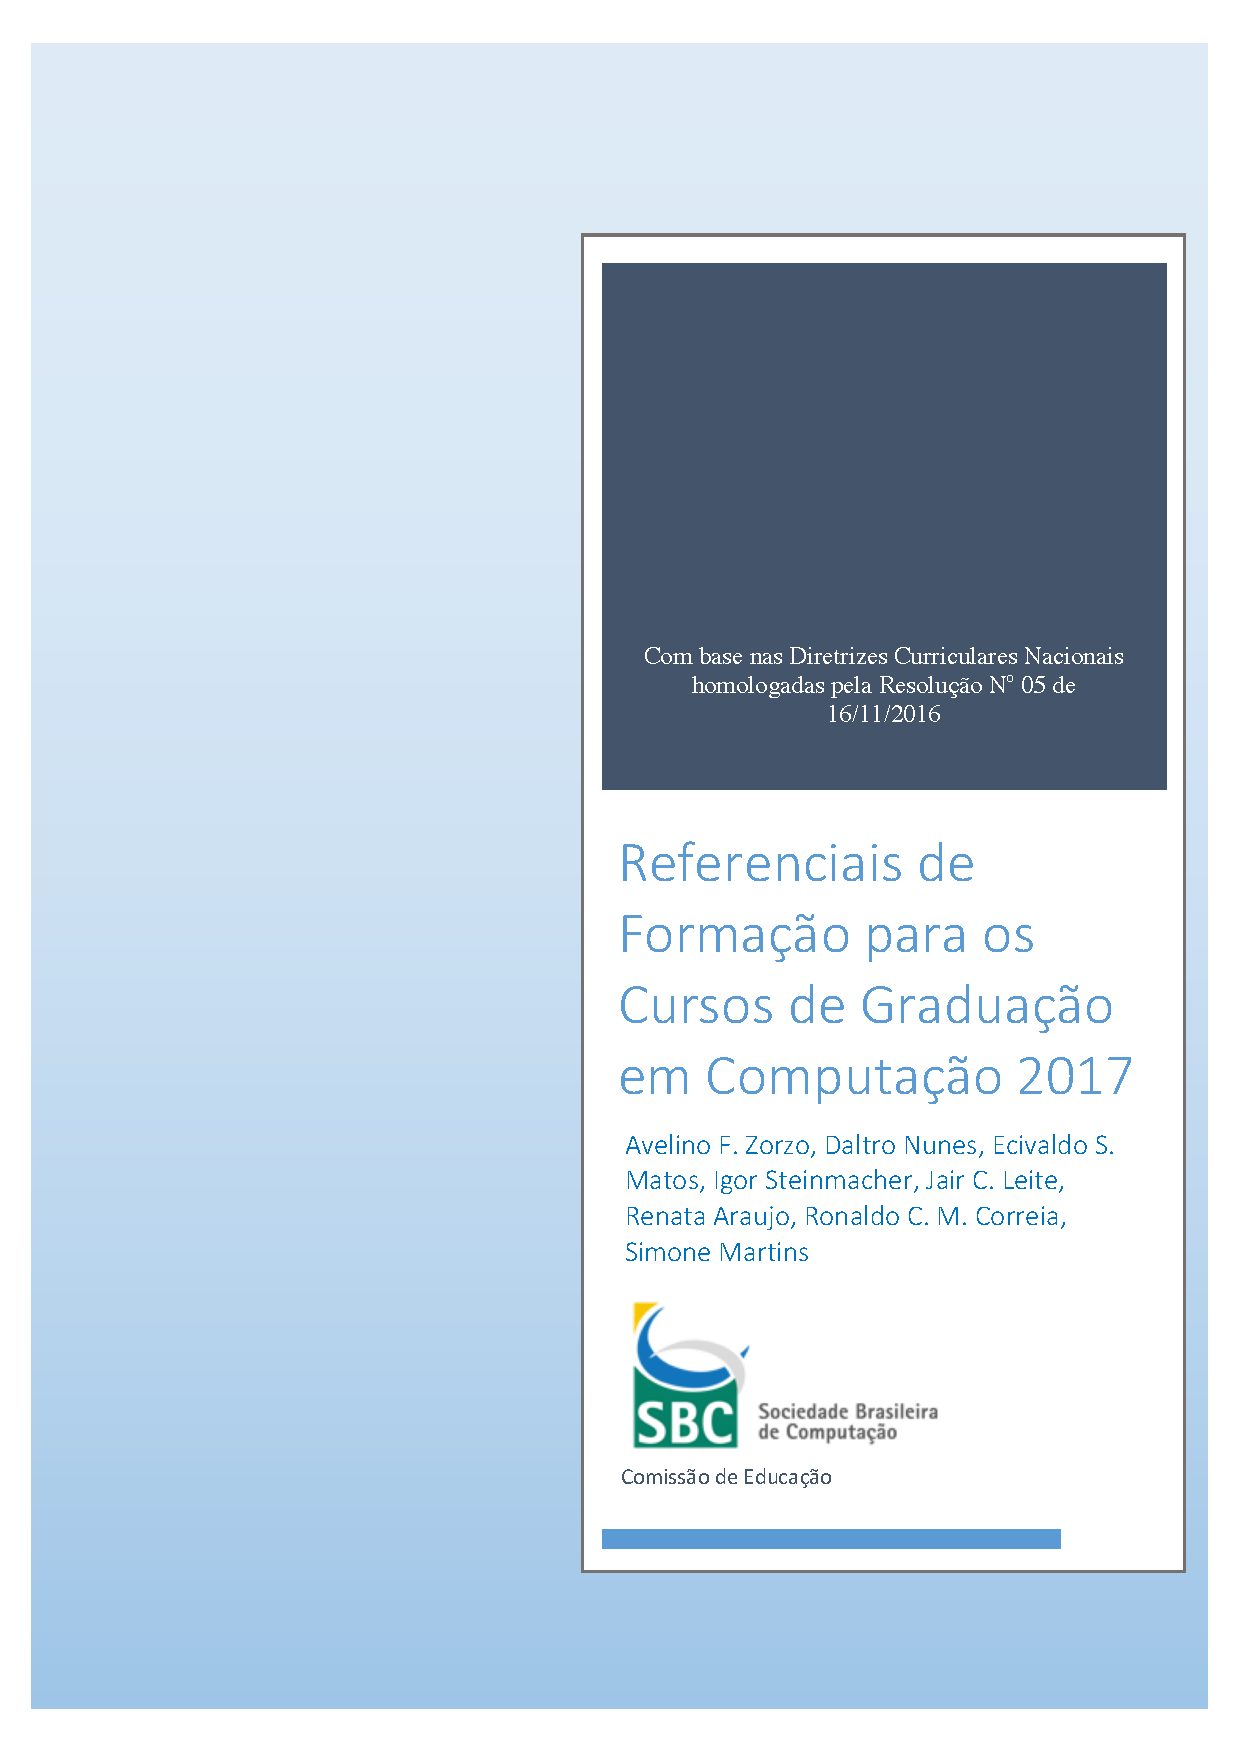
\includepdf[pages=-,pagecommand={\thispagestyle{empty}}]{leis/sbc2017.pdf}
% Resolução CNE/CES n. 7/2018, que estabelece as as Diretrizes para a Extensão na Educação Superior Brasileira
\section{Resolução n\textordmasculine{} 7, de 18 de dezembro de 2018 - CNE/CES}
\label{rcne2018}
\includepdf[pages=-,pagecommand={\thispagestyle{empty}}]{leis/rces007_18.pdf}
% Deliberação n. 33/95, regras gerais de graduação UERJ
\section{Deliberação n\textordmasculine{} 33/95 da UERJ}
\label{delib3395}
\includepdf[pages=-,pagecommand={\thispagestyle{empty}}]{leis/del-uerj1995.pdf}
% Deliberação n. 59/2019 da UERJ que altera a Deliberação n. 33/95 
\section{Deliberação n\textordmasculine{} 59/2019 da UERJ}
\label{delib592019}
\includepdf[pages=-,pagecommand={\thispagestyle{empty}}]{leis/del-uerj2019.pdf}
% Deliberaçao n. 04/2023 do CSEPE/UERJ dispõe sobre inserção curricular da extensão na UERJ
\section{Deliberação n\textordmasculine{} 04/2023 do CSEPE/UERJ}
\label{del4}
\includepdf[pages=-,pagecommand={\thispagestyle{empty}}]{leis/del-uerj2023.pdf}
%  Resolução n. 380/1993 CREA/CONFEA. Discrimina as atribuições do Engenheiro de Computação
\section{Resolução n\textordmasculine{} 380/1993 CREA/CONFEA}
\label{confea1993}
\includepdf[pages=1,pagecommand={\thispagestyle{empty}}]{leis/confea93.pdf}


\end{document}
